\section{Findings, Pitfalls, and Recommendations}

In the spirit of transparency, we discuss key challenges we faced during our training effort, as well as our decision process and thinking for different design decisions. While we have not yet had time to rigorously test some of the hypotheses discussed in this section, we felt sharing them would be valuable as a way of making LM pretraining knowledge explicitly available to the community, and we hope they will benefit future LM pretraining efforts.
Many of the points we discuss here highlight the need for a systematic and open science of pretraining, and we hope they provide promising directions for future work along these lines.

\subsection{Debugging Training Instability}

A recurring problem during our training efforts was debugging training instability: sudden increases in the loss despite a previously smooth downward trend.
Anecdotally, we observed two types of instabilities: sharp sudden spikes and more gradual spikes.

We encountered spikes many different times during our training effort, and there was no simple magic bullet to debug each case.
Yet, we found that a crucial best practice was to plot norm metrics to track the growth of the parameters.
This is motivated by the hypothesis that spikes are related to fast growth rates in the update norms in specific parameters, with sudden growth in the steep case and more gradual, but still too fast, growth for less steep spikes.
The simplest thing to plot is the gradient norm, which indirectly controls the size of an update.
But gradient norms can be noisy, so another easy metric to plot is the parameter norm, which is roughly proportional to the gradient norm \citep{merrill2021effects} but less noisy.
Neither of these metrics would detect issues due to the optimizer state, so we also plot norms of the optimizer state.
Finally, we found that the layer-norm parameters were particularly important for debugging instabilities.

We explored the impact of many architectural decisions on stability in this way.
One of the central anecdotal findings was that removing layer-norm parameters and embedding weight-tying were both particularly helpful for preventing instability.
We speculate below about why this may be the case and plan to investigate it more systematically in future work.

\subsubsection{Removing Weight Tying Improves Stability} \label{sec:instability}

% \begin{figure}
%     \centering
%     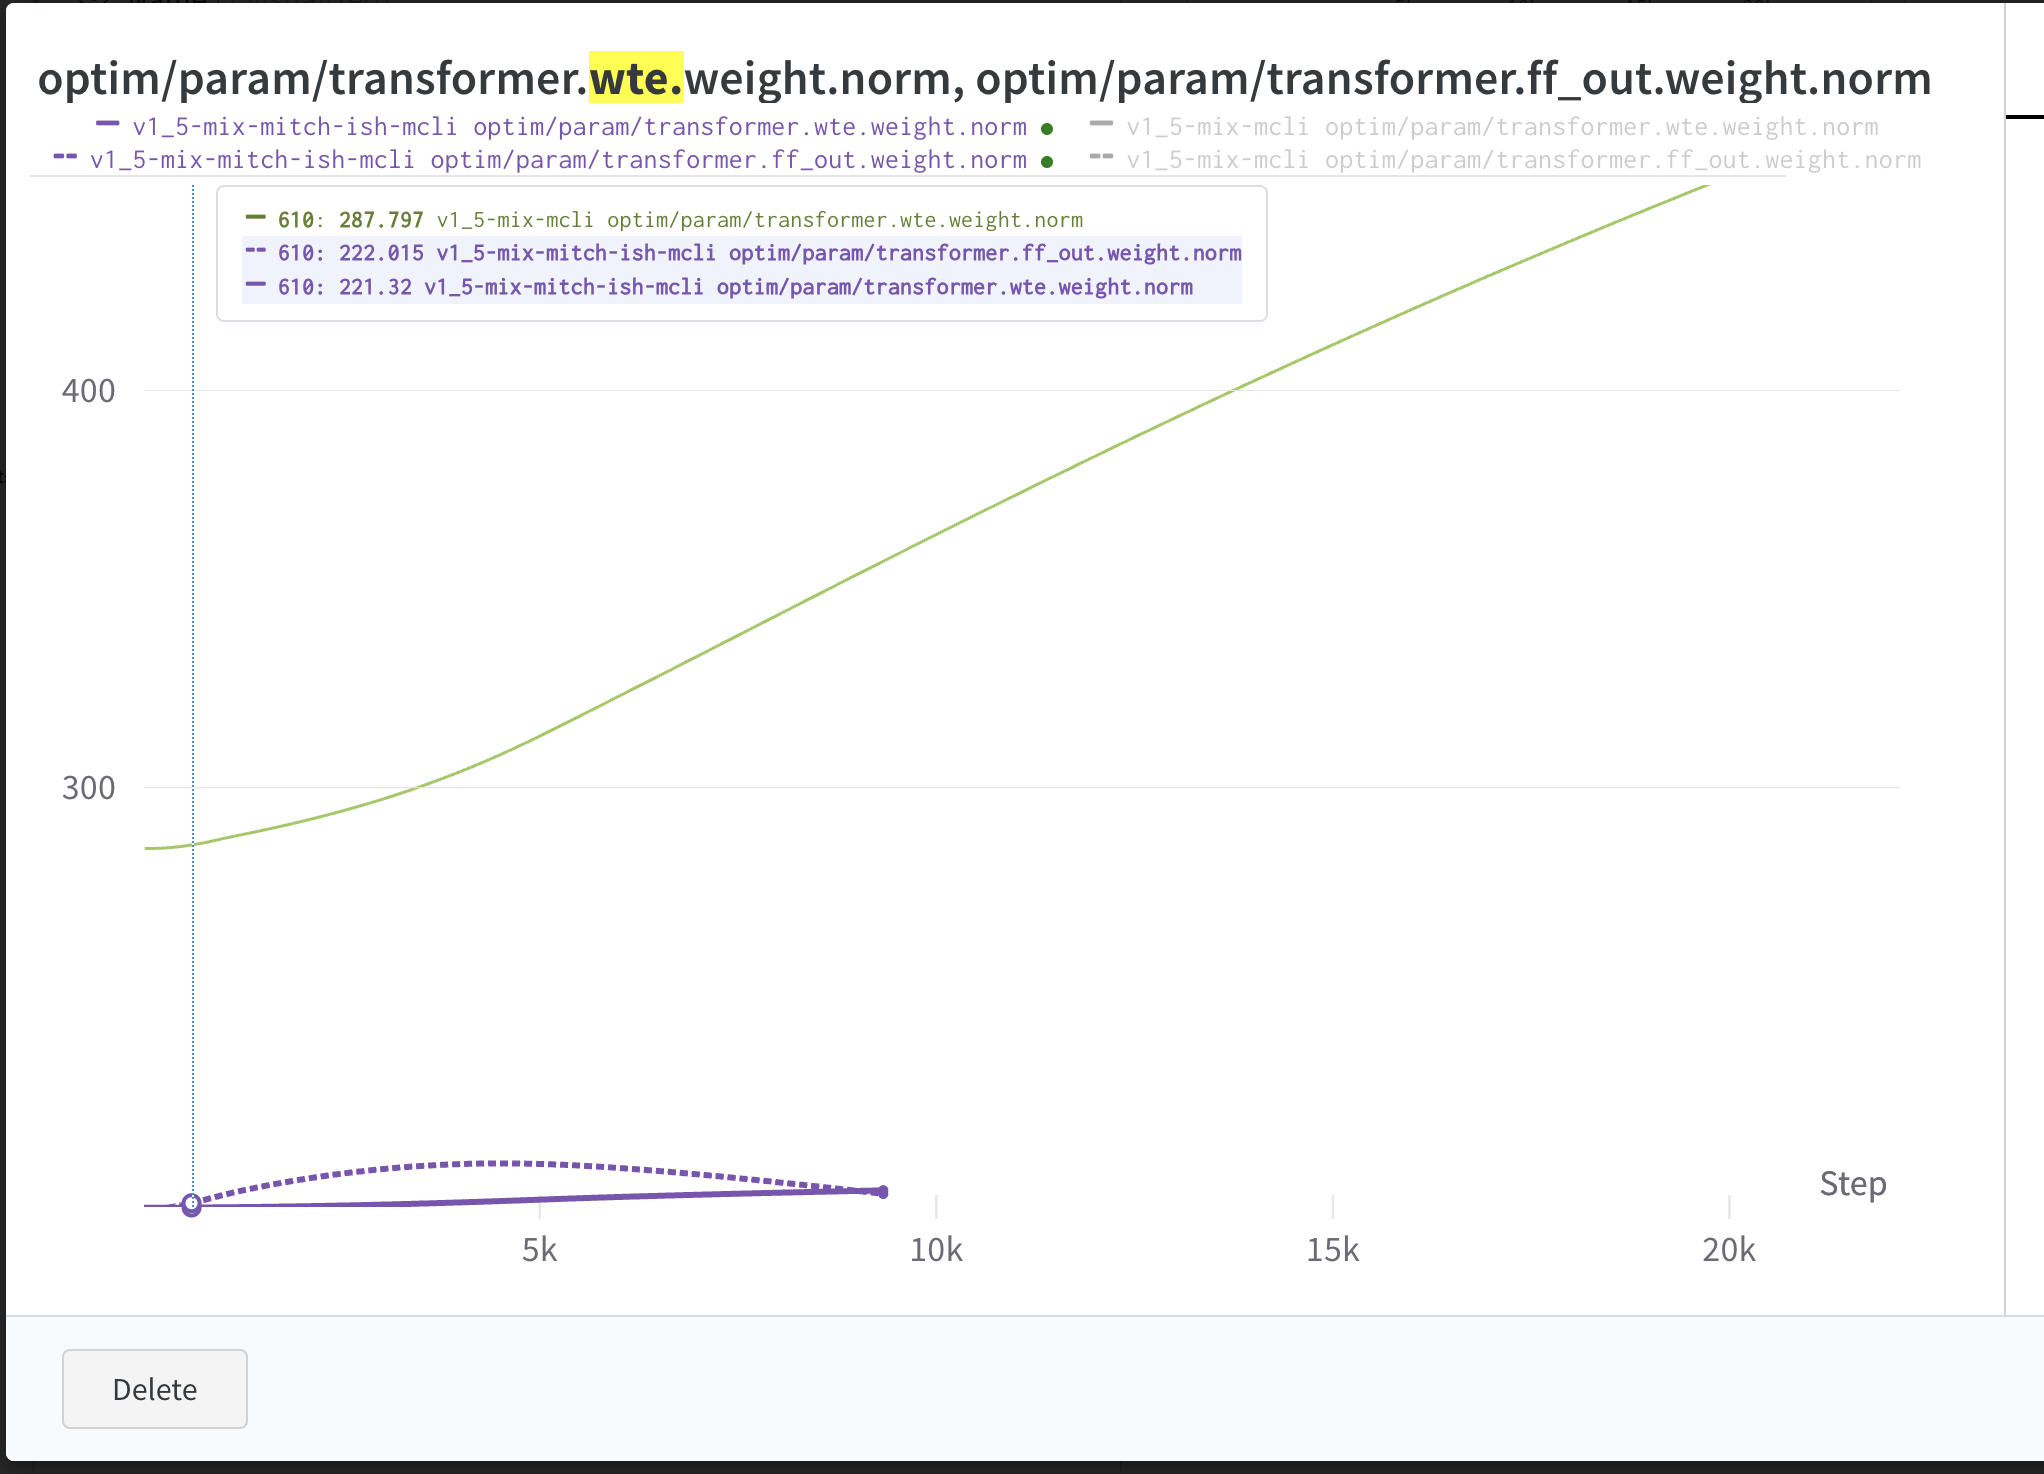
\includegraphics[width=.8\textwidth]{figures/weight-tying-norms.png}
%     \caption{Unembedding parameter norms with and without weight tying. [PLACEHOLDER]}
%     \label{fig:weight-tying}
% \end{figure}

One of our most crucial anecdotal insights in combatting loss spikes was that removing weight-tying of the embedding and unembedding matrices seems to dramatically reduce the frequency and severity of loss spikes. We speculate this is related to the fact that weight tying updates the embedding norms more than they would be updated without weight tying.
In particular, rare tokens will be updated every step for from the final layer but only infrequently from the embedding layer (when those tokens occur in the data).
This means the updates from the final layer may dominate and may cause important features of rare embeddings to be unlearned.
Thus, while weight tying has been beneficial for training smaller languages in the past \citep{press-wolf-2017-using}, we believe it may be counterproductive in the modern large LM regime.

% \willm{copied from loss spikes section here, should merge in}
% We speculate that this may be related to the fact that weight tying grows the parameter norm (and thus gradient norms) of the embedding parameters more than they would grow otherwise. In particular, uncommon embeddings will be updated every step from the final layer but only infrequently from the initial layer, which we believe could cause the model to unlearn features of those tokens.

\subsubsection{Risk of Instability with Lion Optimizer}

The two optimizers we considered using were AdamW \citep{loshchilov2018decoupled} and Lion \citep{chen2023symbolic}. AdamW is a safe and well-tested option. On the other hand, Lion has shown promising gains over AdamW, but we found in preliminary experiments and heard anecdotally that it may run into instability for long training runs.\footnote{For example, this GitHub issue: \url{https://github.com/mlfoundations/open_clip/pull/432}}

Beyond this anecdotal evidence of Lion's instability, we also have a theoretical argument for why Lion would become unstable later in training.
The key property of Lion is the signed update: the parameters are updated by the sign of the step $\sgn(\delta_t)$ rather than the gradient step $\delta_t$ itself.
When the parameters are all on a similar order of magnitude (like at initialization), this should not distort the step direction much.
But \citet{dettmers2022llmint8} show how features with magnitude significantly larger than their neighbors eventually emerge in LMs during training. Assuming the step $\delta_t$ is roughly proportional to the parameters, this means we can get gradient steps on very different orders of magnitude later in training.
Despite this, Lion will update all parameters on the same order of magnitude, e.g.:
\begin{align*}
    % \delta_i = (-.03, .01, 0, -.01) \quad \quad
    % \sgn(\delta_i) = (-1, 1, 1, -1) \\
    \delta_f = (-10, 10^{-1}, 10^{-5}, -10^{-1}) \quad \quad
    \sgn(\delta_f) = (-1, 1, 1, -1)
\end{align*}
This will severely distort the direction of $\sgn(\delta_t)$ compared to $\delta_t$. For example, in the case above we get a cosine similarity of $0.51$. This means that, in the presence of emergent features, we are taking steps in \emph{a different direction} compared to other optimizers, which we expect could lead to instability.

We ultimately chose to use AdamW over Lion so that we could be confident the optimizer would remain stable late into training. However, we believe it would be valuable to explore this theoretical instability issue with Lion more systematically in future work.

\subsubsection{Role of Learning Rate Schedule for Stable Training}

Our hypotheses around instability and gradient norm growth informed our choice of learning rate schedule. We hypothesized that instability is related to exploding growth in the gradient and parameter norms. The learning rate schedule controls the rate at which parameter norms grow, so by calibrating the learning rate schedule appropriately, we can prevent parameters growing too fast and causing a blow up in parameter or gradient norms. On the other hand, we want to learn as efficiently as we can, so we would like to set the learning rate schedule to decay as gradually as possible without causing instability.

We considered several options for the LR schedule and the impact on the parameter growth rate:

\begin{figure}[!t]
    \centering
    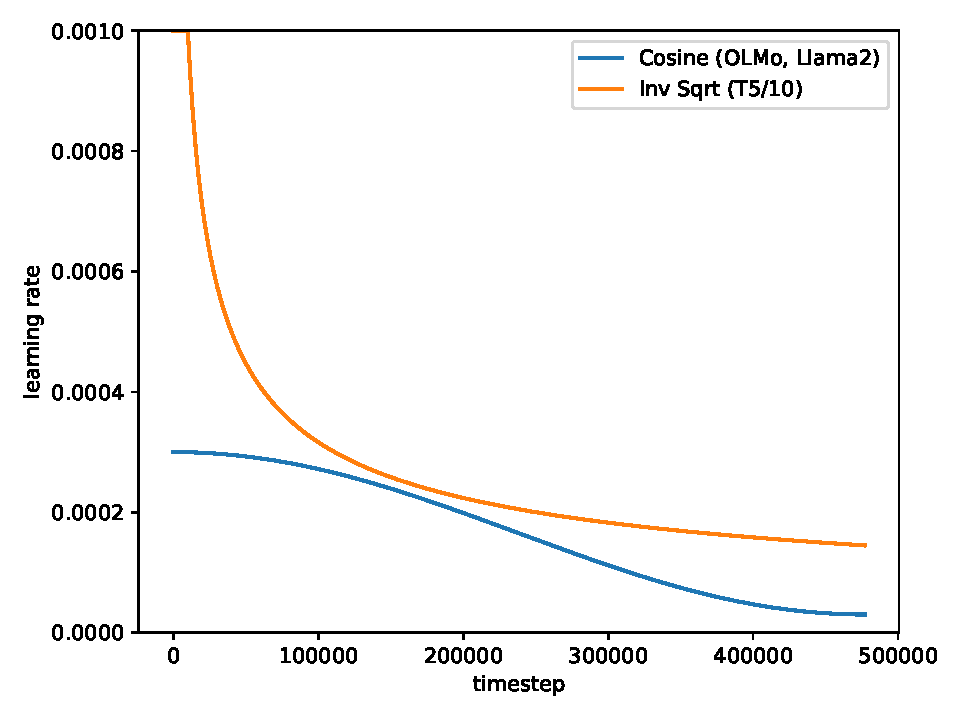
\includegraphics[width=.5\textwidth]{figures/lrs.pdf}
    \caption{
        OLMo cosine schedule vs.~T5 inverse square root schedule with 10\% of its original learning rate.
    }
    \label{fig:lr-schedules}
\end{figure}

\begin{enumerate}
    \item \textbf{Constant Schedule:} This schedule will lead to blow up because the gradient updates will get larger with each step \citep{merrill2021effects}. This suggests we can get exponentially growing gradient norms for parameters that are frequently updated. A model trained with a constant learning rate may look stable for some time, but eventually we expect the gradient norms to blow up, causing instability.
    \item \textbf{Cosine Schedule:} A simple way to prevent such blow up is to decay the learning rate. A common practical choice \citep{biderman2023pythia,touvron2023llama2} for LM pretraining is to use a cosine decay schedule from 100\% to 10\% of the initial learning rate.
    This guarantees that the learning rate decays over time, but requires knowing the maximum number of pretraining steps in advance.
    \item \textbf{Linear Schedule:} Another way to decay the learning rate the learning rate is to simply linearly interpolate between 100\% and 10\%. This is somewhat simpler than the cosine schedule, and will mean slightly smaller learning rates early in training and slightly larger learning rates later.
    \item \textbf{Inverse Square Root Schedule:} A final option is to decay the learning rate proportional to the inverse square root of time. This approach has the advantage that the number of pretraining steps does not need to be fixed in advance, meaning models can be trained longer if more tokens become available, and aiding comparability between models trained on different numbers of tokens.
    We view the inverse square root schedule as less standard than cosine, although it was used by T5 \citep[11B;][]{raffel2020exploring} and PaLM \citep[540B;][]{chowdhery2022palm}. Additionally, \citet{merrill2021effects} provide some theoretical support for the inverse square root schedule.
\end{enumerate}

We ultimately chose the linear schedule out of a combination of simplicity and conservatism. 
With an appropriate initial learning rate,
cosine and linear can both be made strictly more conservative than the inverse square root schedule, as shown in \Cref{fig:lr-schedules}.
Compared to cosine, the linear schedule is simpler and does not decay so extremely later in training.

For future LM training efforts, we believe that better understanding of learning rate schedules could very well lead to different decisions than what we made.
In particular, we were tempted to try an inverse square root schedule but ultimately chose against it because we were not entirely sure training would remain stable.
Better theories of stability rooted in optimization would make it much easier to make these decisions.

\subsection{Engineering Challenges and Best Practices}
\people{Dirk, Pete}

Multi GPU, precision, etc.

\begin{enumerate}
    \item Parameter dimensions should be multiples of 256, including the embedding matrix to increase GPU throughput
    \item fp32, reduce, etc.
    \item FSDP
\end{enumerate}

\willm{Possibly mention layer norm and QK norm here}

\subsection{Interesting Observations}

\people{Dirk}

\begin{enumerate}
    \item (Nov 1) Some OLMo and OpenLM configs did well without positional embeddings. Related to the fact that decoder models can reconstruct position without positional embeddings? Could we look into removing positional embeddings in the future? Would it help with length generalization?
    \willm{Think we drop this, or make it a brief one liner and cite existing work on models without positional embeddings (e.g., NoPE, one of OfirP's papers, Eleuther paper)}

    \item PyTorch's random permutation function is not random enough for shuffling large datasets. \petew{TODO - copy over text and graphs from our LOG.md file}

    \item If the dataset is not IID, bad things happen    

    \item Alibi doesn't see positions that are further than 256 tokens

    \item ...
\end{enumerate}